\documentclass{beamer}
\usetheme{}
\usecolortheme{dolphin}           
\useinnertheme{circles}
\setbeamertemplate{itemize items}[default]
\setbeamertemplate{enumerate items}[default]
\usepackage[T1]{fontenc}
\usepackage[utf8]{inputenc}
\usepackage{lmodern}
\usepackage{amsmath}
\usepackage{booktabs} 
\usepackage{graphicx}        
\usepackage{array}
\usepackage{color}
\makeatletter
\def\zapcolorreset{\let\reset@color\relax\ignorespaces}
\def\colorrows#1{\noalign{\aftergroup\zapcolorreset#1}\ignorespaces}
\makeatother
\graphicspath{{/home/swl/Dropbox/ucd/advanced_macro/figures/}} 
\setbeamertemplate{navigation symbols}{}
\setbeamertemplate{footline}[frame number]
%--------------------------------------
\title{Kalman filter}
\author{School of Economics, University College Dublin}
\date{Spring 2018}
\begin{document}

%--------------------------------------
\begin{frame}
 \titlepage
\end{frame}
%--------------------------------------

%--------------------------------------
\begin{frame}
  \textbf{Latent variables:} Variables that are not directly observed but inferred from other variables
  \begin{itemize}
    \item Unobserved, but variable can still play important role in theoretical model
  \end{itemize}
  \medskip
  Example: Potential output
  \begin{itemize}
    \item Keynesian model: inflationary pressure determined by deviation of output from potential output
    \item Consider GDP increase in last quarter but no sign of inflationary pressure: potential output increased
  \end{itemize}  
  \medskip
  \textbf{Q:} Can we assume that there has been a change in potential output?
\end{frame}
%--------------------------------------

%--------------------------------------
\begin{frame}
  \textbf{A:} Potential output probably stable from quarter to quarter while there is likely random noise fluctuations in inflation
  \begin{itemize}
    \item Signal vs. noise: Need to have a method that extracts useful signal from data that also contains lot of noise
  \end{itemize}
  \medskip  
   One way to extract a signal is the \textbf{Kalman filter}
   \begin{itemize}
     \item Recursive method to estimate state of process; minimises MSE
   \end{itemize}
\end{frame}
%--------------------------------------

%--------------------------------------
\begin{frame}
  \textbf{Conditional expectations:}\\
   We want an estimate of the value of variable $X$ 
  \begin{itemize}
    \item Problem: we don't observe $X$
  \end{itemize}
  \medskip
  Do observe $Z$ which is correlated with $X$: Assume that $X,Z$ are jointly normally distributed
  \begin{align}
    \begin{pmatrix}      X \\Z     \end{pmatrix}
    \sim N \left ( \begin{pmatrix}      \mu_X \\ \mu_Z    \end{pmatrix},
    \begin{pmatrix}       \sigma^2_X & \sigma_{XZ} \\ \sigma_{XZ} & \sigma^2_Z     \end{pmatrix} \right )
  \end{align}  
  \medskip
  We get
  \begin{align}
    \mathbb{E}(X|Z) = \mu_X + \frac{\sigma_{XZ}}{\sigma^2_Z}(Z-\mu_Z)
  \end{align}
\end{frame}
%--------------------------------------

% Need to check this slide
%--------------------------------------
\begin{frame}
  Alternatively, define $\rho$ as correlation between $X$ and $Z$
  \begin{align}
    \rho= \frac{\sigma_{XZ}}{\sigma_X \sigma_Z}
  \end{align}
  Inserting in (2) we get
  \begin{align}
    \mathbb{E}(X|Z) = \mu_X + \rho \frac{\sigma_X}{\sigma_Z}(Z-\mu_Z)
  \end{align}
  \medskip
  Weight put on information from $Z$ depends on
  \begin{enumerate}
    \item Correlation between $X$ and $Z$ ($\rho$)
    \item The relative standard deviation ($\frac{\sigma_X}{\sigma_Z}$)
  \end{enumerate}
  If $Z$ has high standard deviation, it is a poor signal.
\end{frame}
%--------------------------------------

%--------------------------------------
\begin{frame}
  \textbf{Multivariate conditional expectations}\\
  Can generalise from 2 to $n$ variables
  \begin{itemize}
    \item Let $X$ be $1\; x\; n$ vector of variables and $Z$ $1\; x\; m$ 
  \end{itemize}  
  \begin{align}
    \begin{pmatrix}      X \\ Z    \end{pmatrix} \sim N \left( 
    \begin{pmatrix}      \mu_X \\ \mu_Z    \end{pmatrix},
    \begin{pmatrix}      \sum_{XX} & \sum_{XZ} \\ \sum_{XZ}' & \sum_{ZZ}    \end{pmatrix}
    \right)
  \end{align}
  \medskip 
  Expected value of $X$ conditional on $Z$ is 
  \begin{align}
    \mathbb{E}(X|Z) = \mu_X + \scriptstyle \sum_{XZ}\sum^{-1}_{ZZ} \textstyle(Z-\mu_Z)
  \end{align}  
\end{frame}
%--------------------------------------

%--------------------------------------
\begin{frame}
  \textbf{State-space models:} Linear time-series models that mix observable and unobservable variables.
  \begin{align}
    S_t=FS_{t-1} + u_t
  \end{align}
  \textbf{State equation} - or transition equation - describes how unobservables $S_t$ evolve over time
  \begin{align}
    Z_t= HS_t +v_t
  \end{align}
  \textbf{Measurement equation}, relates set of observable variables $Z_t$ to unobservable variables $S_t$    
\end{frame}
%--------------------------------------

%--------------------------------------
\begin{frame}
  \textbf{Errors:} Both $u_t$ and $v_t$ can include either 
  \begin{enumerate}
    \item Normally distributed errors
    \item Zeros, if the described equation is an identity
  \end{enumerate}
  \begin{align}
    u_t &\sim N(0,\scriptstyle \sum^u) \\
    v_t &\sim N(0,\scriptstyle \sum^v)
  \end{align}
  \medskip
  $\sum$ might not have full matrix rank
  \begin{itemize}
    \item Or rank deficient
    \item i.e. not enough information in data to estimate equation
  \end{itemize}  
\end{frame}
%--------------------------------------

%--------------------------------------
\begin{frame}
  \textbf{Estimation:} Observed data described by
  \begin{align}
    Z_t = HS_t + v_t
  \end{align}
  Cannot observe $S_t$ but can replace it with unbiased guess based on information available at time $t$
  \begin{align}
    S_{t|t-1}
  \end{align}
  Assume that errors are normally distributed with known covariance matrix
  \begin{align}
    S_t-S_{t|t-1} \sim N (0,\scriptstyle \sum^S_{t|t-1} \textstyle)
  \end{align}
  Can express observed variables as
  \begin{align}
    Z_t=HS_{t|t-1}+v_t +H(S_t-S_{t|t-1})
  \end{align}
\end{frame}



%--------------------------------------
\begin{frame}
  \begin{itemize}
     \item $S_{t|t-1}$ is observable
     \item $v_t, S_t-S_{t|t-1}$ are unobservable but normally distributed
   \end{itemize} 
  Can estimate model using ML ; with observed data
  \begin{align}
    Z_t=HS_{t|t-1}+v_t +H(S_t-S_{t|t-1})
  \end{align}
  Variance of error , after conditioning on $t-1$ state-variable estimate, is given by
  \begin{align}
    v_t &+ H(S_t-S_{t|t-1}) \sim N (0,\Omega_t)\\
    \Omega_t &=\scriptstyle\sum^v +H\sum^S_{t|t-1}H'
  \end{align}  
\end{frame}
%--------------------------------------

%--------------------------------------
\begin{frame}
  Parameters of model are given by 
  \begin{align}
    \theta=(F,H,\scriptstyle \sum^u,\sum^v \textstyle)
  \end{align}
  Log-likelihood function for $Z_t$ given observables at $t-1$ is  
  \begin{align}
    log\;f(Z_t|Z_{t-1},\theta)&= -log\; 2\pi -log\;|\Omega_t|- \\ \nonumber &\frac{1}{2}(Z_t-HS_{t|t-1})' \Omega_t^{-1}(Z_t-HS_{t|t-1})
  \end{align}  
\end{frame}
%--------------------------------------



%--------------------------------------
\begin{frame}
  Combined likelihood is given by
  \begin{itemize}
    \item Based on initial estimate of first period unobservable state $S_{1|0}$
  \end{itemize}
  \begin{align}
    f(Z_1,...,Z_T|S_{1|0},\theta)=f(Z_1|S_{1|0},\theta)\prod_{i=2}^{i=T}f(Z_i|Z_{i-1},\theta)
  \end{align}
  \begin{align}
    log\;f(Z_1,...,Z_T|S_{1|0}, \theta) &= -T\;log\; 2\pi - \sum^T_{i=2}log\; |\Omega| \\ \nonumber
    &- \frac{1}{2} \sum^T_{i=1} (Z_i-HS_{i|i-1})' \Omega_i^{-1} (Z_i - HS_{i|i-1}) 
  \end{align}
  ML parameter estimates will be set of matrices $\theta=(F,H,\sum^v,\sum^u)$ that provides largest value for this function  
\end{frame}
%--------------------------------------

%--------------------------------------
\begin{frame}
  MLE will estimate model's parameters; only need an unbiased guess based on information available at $t-1$ ($S_{t|t-1}$): Use Kalman filter 
  \begin{itemize}
    \item Iterative method
    \item Provides estimates of state variables for $t$, uses observable data for $t+1$ to update estimates
  \end{itemize}
\end{frame}
%--------------------------------------

%--------------------------------------
\begin{frame}
  \textbf{Estimating state variables:} Formulate estimate of state variable at time $t$ given information at $t-1$
  \begin{align}
    S_t=FS_{t-1}+u_t \Rightarrow S_{t|t-1}=FS_{t-1|t-1}
  \end{align}
  At $t-1$, expected value for the observables at $t$ are
  \begin{align}
    Z_{t|t-1}=HS_{t|t-1}=HFS_{t-1|t-1}
  \end{align}
  At $t$ we observe $Z_t$; need to update estimate of state variable given information
  \begin{align}
     Z_t-HFS_{t-1|t-1}
   \end{align} 
\end{frame}
%--------------------------------------

%--------------------------------------
\begin{frame}
  Model assumptions imply
  \begin{align}
    \begin{pmatrix}      S_t \\ Z_t     \end{pmatrix} \sim N \left( 
    \begin{pmatrix}      FS_{t-1|t-1} \\HFS_{t-1|t-1}    \end{pmatrix},
    \begin{pmatrix}      \sum^S_{t|t-1} & \left( H\sum^S_{t|t-1} \right)' \\ H\sum^S_{t|t-1} & \sum^V+H\sum^S_{t|t-1}H' \end{pmatrix} \right)
  \end{align}
  \medskip
  Use conditional expectations to state that minimum variance unbiased estimate of $S_t|Z_t$ is
  \begin{align}
     \mathbb{E}(S_t|Z_t)&=S_{t|t}=FS_{t-1|t-1}+K_t(Z_t-HFS_{t-1|t-1})     
  \end{align}  
\end{frame}
%--------------------------------------

%--------------------------------------
\begin{frame}
  $K_t$ is the \textbf{Kalman gain} matrix
  \begin{align}
    K_t&= \left(H\scriptstyle \sum^S_{t|t-1} \right)' \left( \scriptstyle \sum^V + H\scriptstyle \sum^S_{t|t-1} \textstyle H'\right )^{-1} 
  \end{align}
  \medskip
  Covariance matrices required to compute $K_t$ are updated by 
  \begin{align}
    \scriptstyle \sum^S_{t|t-1} \textstyle &= F\scriptstyle \sum^S_{t-1|t-1}\textstyle F'+ \scriptstyle\sum^U\\
    \scriptstyle \sum^S_{t|t} \textstyle &= (I-K_tH)\scriptstyle \sum^S_{t|t-1}
  \end{align}
\end{frame}
%--------------------------------------


%--------------------------------------
\begin{frame}
  Initialising the Kalman filter we still need
  \begin{enumerate}
    \item Initial estimate $S_{1|0}$
    \item Covariance matrix
  \end{enumerate}
  \medskip
  In many macroeconomic models $S$ can be assumed to have zero mean. For the covariance matrix we use
  \begin{align}
    \scriptstyle \sum^S_{t|t-1} = \textstyle F \scriptstyle \sum^S_{t-1|t-1} \textstyle F' + \scriptstyle \sum^u
  \end{align}
  Values of this covariance matrix will converge; for unconditional covariance matrix can use value for $\sum$ that solves
  \begin{align}
    \scriptstyle \sum=\textstyle F \scriptstyle \sum \textstyle F' + \scriptstyle \sum^u
  \end{align}
\end{frame}
%--------------------------------------

%--------------------------------------
\begin{frame}
  \textbf{Kalman smoother:} Kalman filter is a one-sided filter
  \begin{itemize}
    \item $\hat{S}_t$ based on data available at $t$ 
  \end{itemize}
  \medskip
  Good for real-time, but we often have access to full historical dataset
  \begin{itemize}
    \item Time-varying models can be estimated using Kalman smoother
    \item Two-sided filter using all available data to compute $\hat{S}_t$
  \end{itemize}  
\end{frame}
%--------------------------------------

%--------------------------------------
\begin{frame}
  \textbf{Hodrick-Prescott filter}
  \begin{align}
    \sum_{t=1}^{N} [(y_t - y_t^*)^2+ \lambda(\Delta y_t^* - \Delta y_{t-1}^*)]
  \end{align}
  Consider state-space model
  \begin{align}
    y_t &= y^*_t+C_t\\
    \Delta y^*_t &= \Delta y^*_{t-1} + \epsilon^g_t \\
    C_t &= \epsilon_t^c
  \end{align}
  Here
  \begin{align}
    Var(\epsilon^g_t) &= \sigma_g^2; Var(\epsilon_t^c) = \sigma_c^2
  \end{align}
  HP filter = Kalman filter when
  \begin{align}
    \lambda = \frac{\sigma_c^2}{\sigma_g^2} 
  \end{align}
  It is assumed that $\sigma_c^2$ is 5 percentage points and $\sigma_g^2$ one-eight percentage point: $\lambda=1600$
\end{frame}
%--------------------------------------

%--------------------------------------
\begin{frame}
  \textbf{Laubach \& Williams} (2001): Estimate model with two unobservable time-varying series
  \begin{enumerate}
    \item Potential output
    \item Natural rate of interest
  \end{enumerate}
  \begin{align*}
    \tilde{y}_t &= y_t-y^*_t \\ 
    \tilde{y}_t &= A_y(L)\tilde{y}_{t-1} + A_r(L)(r_{t-1}-r^*_{t-1}) + \epsilon_{1t}\\
    \pi_t &= B_{\pi}(L)\pi_{t-1} + B_y(L)\tilde{y}_{t-1} + B_x(L)x_t + \epsilon_{2t}\\
    r^*_t &= cg_t +z_t\\
    z_t &= D_z(L)z_{t-1} + \epsilon_{3t}\\
    y^*_t &= y^*_{t-1} +g_{t-1} + \epsilon_{4t}\\
    g_t &= g_{t-1} + \epsilon_{5t}
  \end{align*}
\end{frame}
%--------------------------------------

%--------------------------------------
\begin{frame}
  \begin{figure}
    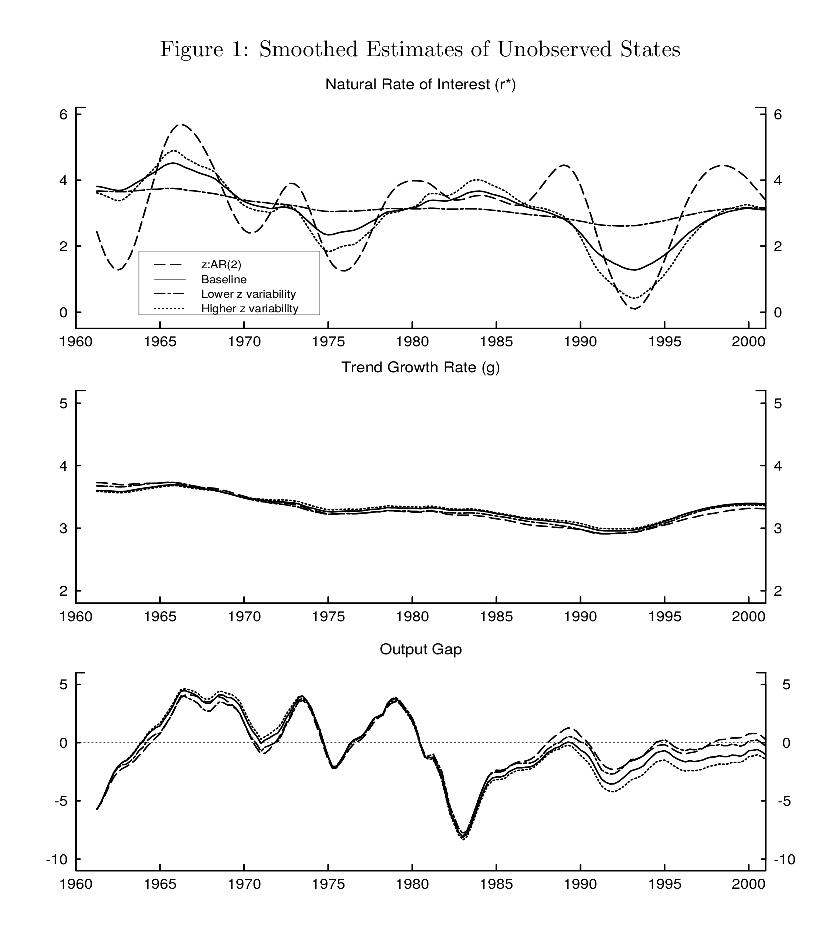
\includegraphics[scale=.5]{lw.eps}
  \end{figure}
\end{frame}
%--------------------------------------

%--------------------------------------
\begin{frame}
  \begin{figure}
    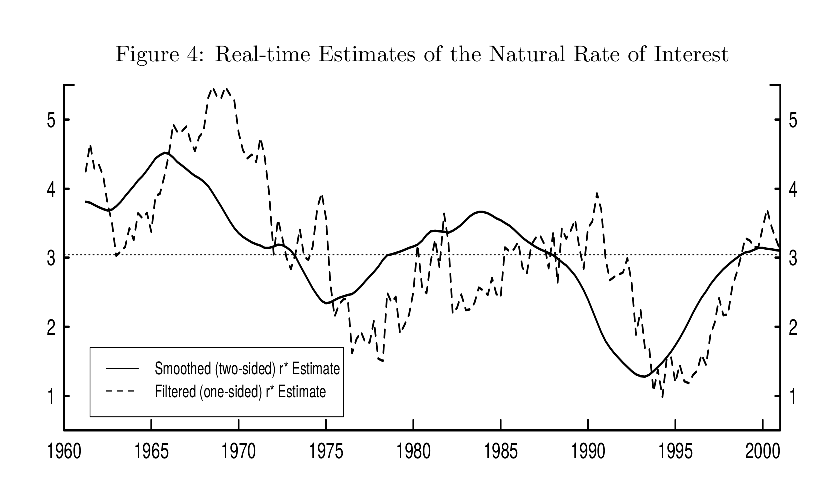
\includegraphics[scale=.7]{lw2.eps}
  \end{figure}
\end{frame}
%--------------------------------------



%--------------------------------------
\end{document}
